\documentclass[11pt,a4paper]{report}
\usepackage[textwidth=37em,vmargin=30mm]{geometry}
\usepackage{calc,xunicode,amsmath,amssymb,paralist,enumitem,tabu,booktabs,datetime2,xeCJK,xeCJKfntef,listings}
\usepackage{tocloft,fancyhdr,tcolorbox,xcolor,graphicx,eso-pic,xltxtra,xelatexemoji}

\newcommand{\envyear}[0]{2024}
\newcommand{\envdatestr}[0]{2024-11-09}
\newcommand{\envfinaldir}[0]{webdb/2024/20241109/final}

\usepackage[hidelinks]{hyperref}
\hypersetup{
    colorlinks=false,
    pdfpagemode=FullScreen,
    pdftitle={Web Digest - \envdatestr}
}

\setlength{\cftbeforechapskip}{10pt}
\renewcommand{\cftchapfont}{\rmfamily\bfseries\large\raggedright}
\setlength{\cftbeforesecskip}{2pt}
\renewcommand{\cftsecfont}{\sffamily\small\raggedright}

\setdefaultleftmargin{2em}{2em}{1em}{1em}{1em}{1em}

\usepackage{xeCJK,xeCJKfntef}
\xeCJKsetup{PunctStyle=plain,RubberPunctSkip=false,CJKglue=\strut\hskip 0pt plus 0.1em minus 0.05em,CJKecglue=\strut\hskip 0.22em plus 0.2em}
\XeTeXlinebreaklocale "zh"
\XeTeXlinebreakskip = 0pt


\setmainfont{Brygada 1918}
\setromanfont{Brygada 1918}
\setsansfont{IBM Plex Sans}
\setmonofont{JetBrains Mono NL}
\setCJKmainfont{Noto Serif CJK SC}
\setCJKromanfont{Noto Serif CJK SC}
\setCJKsansfont{Noto Sans CJK SC}
\setCJKmonofont{Noto Sans CJK SC}

\setlength{\parindent}{0pt}
\setlength{\parskip}{8pt}
\linespread{1.15}

\lstset{
	basicstyle=\ttfamily\footnotesize,
	numbersep=5pt,
	backgroundcolor=\color{black!5},
	showspaces=false,
	showstringspaces=false,
	showtabs=false,
	tabsize=2,
	captionpos=b,
	breaklines=true,
	breakatwhitespace=true,
	breakautoindent=true,
	linewidth=\textwidth
}






\newcommand{\coverpic}[2]{
    % argv: itemurl, authorname
    Cover photo by #2~~(\href{#1}{#1})
}
\newcommand{\makeheader}[0]{
    \begin{titlepage}
        % \newgeometry{hmargin=15mm,tmargin=21mm,bmargin=12mm}
        \begin{center}
            
            \rmfamily\scshape
            \fontspec{BaskervilleF}
            \fontspec{Old Standard}
            \fontsize{59pt}{70pt}\selectfont
            WEB\hfill DIGEST
            
            \vfill
            % \vskip 30pt
            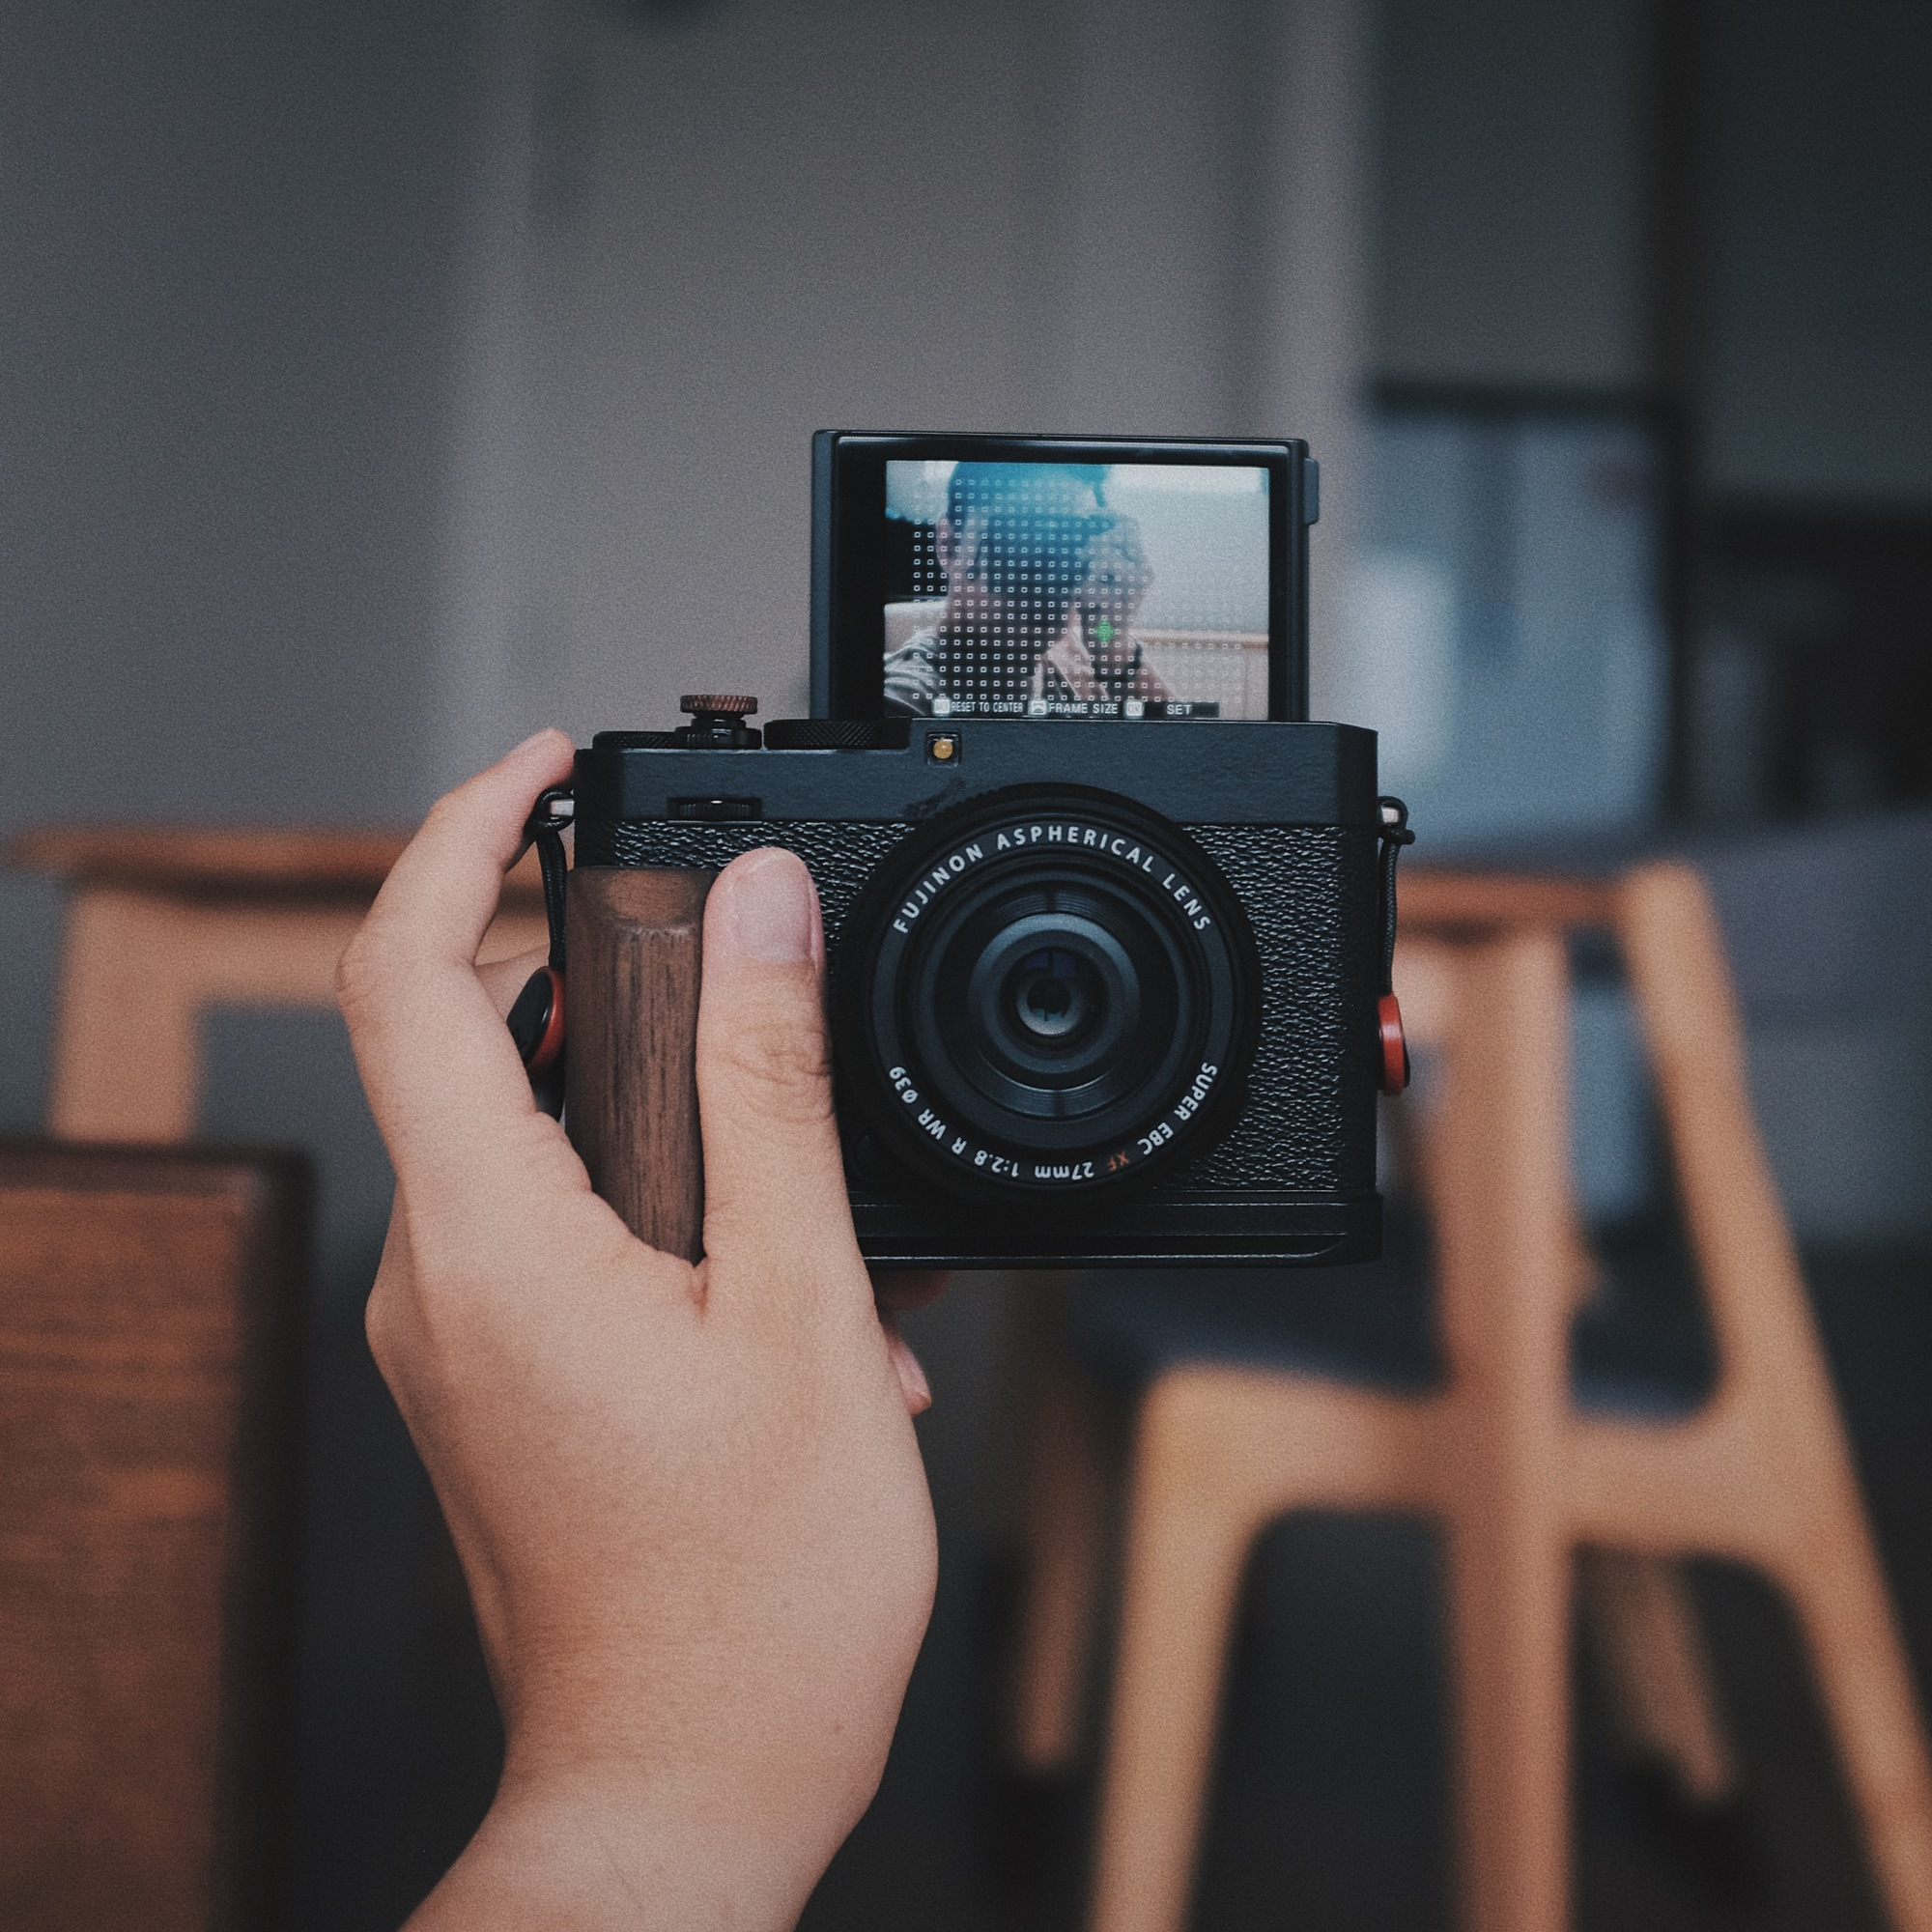
\includegraphics[width=\linewidth]{\envfinaldir/coverpic-prod.jpg}\par
            % \vskip 30pt
            \vfill

            \normalsize\rmfamily\scshape
            \copyright{} The Web Digest Project \hfill\large \envdatestr
        \end{center}
    \end{titlepage}
    % \restoregeometry
}
\newcommand{\simplehref}[1]{%
    \textcolor{blue!80!green}{\href{#1}{#1}}%
}
\renewcommand{\contentsname}{\center\Huge\sffamily\bfseries Contents\par\vskip 20pt}
\newcounter{ipartcounter}
\setcounter{ipartcounter}{0}
\newcommand{\ipart}[1]{
    % \vskip 20pt
    \clearpage
    \stepcounter{ipartcounter}
    \phantomsection
    \addcontentsline{toc}{chapter}{#1}
    % \begin{center}
    %     \Huge
    %     \sffamily\bfseries
    %     #1
    % \end{center}
    % \vskip 20pt plus 7pt
}
\newcounter{ichaptercounter}
\setcounter{ichaptercounter}{0}
\newcommand{\ichapter}[1]{
    % \vskip 20pt
    \clearpage
    \stepcounter{ichaptercounter}
    \phantomsection
    \addcontentsline{toc}{section}{\numberline{\arabic{ichaptercounter}}#1}
    \begin{center}
        \Huge
        \sffamily\bfseries
        #1
    \end{center}
    \vskip 20pt plus 7pt
}
\newcommand{\entrytitlefont}[1]{\subsection*{\raggedright\Large\sffamily\bfseries#1}}
\newcommand{\entryitemGeneric}[2]{
    % argv: title, url
    \parbox{\linewidth}{
        \entrytitlefont{#1}\par\vskip 5pt
        \footnotesize\ttfamily\mdseries
        \simplehref{#2}
    }\vskip 11pt plus 11pt minus 1pt
}
\newcommand{\entryitemGithub}[3]{
    % argv: title, url, desc
    \parbox{\linewidth}{
        \entrytitlefont{#1}\par\vskip 5pt
        \footnotesize\ttfamily\mdseries
        \simplehref{#2}\par\vskip 5pt
        \small\rmfamily\mdseries#3
    }\vskip 11pt plus 11pt minus 1pt
}
\newcommand{\entryitemAp}[3]{
    % argv: title, url, desc
    \parbox{\linewidth}{
        \entrytitlefont{#1}\par\vskip 5pt
        \footnotesize\ttfamily\mdseries
        \simplehref{#2}\par\vskip 5pt
        \small\rmfamily\mdseries#3
    }\vskip 11pt plus 11pt minus 1pt
}
\newcommand{\entryitemHackernews}[3]{
    % argv: title, hnurl, rawurl
    % \parbox{\linewidth}{
    %     \entrytitlefont{#1}\par\vskip 5pt
    %     \footnotesize\ttfamily\mdseries
    %     \simplehref{#3}\par
    %     \textcolor{black!50}{\href{#2}{#2}}
    % }\vskip 11pt plus 11pt minus 1pt
    \begin{minipage}{\linewidth}
            \entrytitlefont{#1}\par\vskip 5pt
            \footnotesize\ttfamily\mdseries
            \simplehref{#3}\par
            \textcolor{black!50}{\href{#2}{#2}}
    \end{minipage}\par\vskip 11pt plus 11pt minus 1pt
}







\begin{document}

\makeheader

\tableofcontents\clearpage




\ipart{Developers}
\ichapter{Hacker News}
\entryitemTwoLinks{Mitochondria Are Alive}{https://news.ycombinator.com/item?id=42088758}{https://www.asimov.press/p/mitochondria}

\entryitemTwoLinks{The Weeds Are Winning}{https://news.ycombinator.com/item?id=42087770}{https://www.technologyreview.com/2024/10/10/1105034/weeds-climate-change-genetic-engineering-superweeds-food/}

\entryitemTwoLinks{Perceptually lossless (talking head) video compression at 22kbit/s}{https://news.ycombinator.com/item?id=42084977}{https://mlumiste.com/technical/liveportrait-compression/}

\entryitemTwoLinks{Principles for product velocity}{https://news.ycombinator.com/item?id=42084753}{https://ssoready.com/blog/from-the-founders/methodology-is-bullshit/}

\entryitemTwoLinks{Multiple new macOS sandbox escape vulnerabilities}{https://news.ycombinator.com/item?id=42084588}{https://jhftss.github.io/A-New-Era-of-macOS-Sandbox-Escapes/}

\entryitemTwoLinks{Rust for tokenising and parsing}{https://news.ycombinator.com/item?id=42083547}{https://xnacly.me/posts/2024/rust-pldev/}

\entryitemTwoLinks{FDA proposes ending use of oral phenylephrine as OTC nasal decongestant}{https://news.ycombinator.com/item?id=42082998}{https://www.fda.gov/news-events/press-announcements/fda-proposes-ending-use-oral-phenylephrine-otc-monograph-nasal-decongestant-active-ingredient-after}

\entryitemTwoLinks{Cops suspect iOS 18 iPhones are communicating to force reboots}{https://news.ycombinator.com/item?id=42081874}{https://www.macrumors.com/2024/11/07/ios-18-forcing-reboots-law-enforcement/}

\entryitemTwoLinks{Ambulance hits cyclist, rushes him to hospital, then sticks him with \$1,800 bill}{https://news.ycombinator.com/item?id=42081764}{https://www.oregonlive.com/pacific-northwest-news/2024/11/ambulance-hits-oregon-cyclist-rushes-him-to-hospital-then-sticks-him-with-1800-bill-lawsuit-says.html}

\entryitemTwoLinks{Trump's likely FCC chair wrote Project 2025 chapter on how he'd run the agency}{https://news.ycombinator.com/item?id=42081726}{https://arstechnica.com/tech-policy/2024/11/trumps-likely-fcc-chair-wrote-project-2025-chapter-on-how-hed-run-the-agency/}

\entryitemTwoLinks{Toronto crypto company CEO kidnapped, held for \$1M ransom before being released}{https://news.ycombinator.com/item?id=42080821}{https://www.cbc.ca/news/canada/toronto/kidnapping-toronto-businessman-cryptocurrency-1.7376679}

\entryitemTwoLinks{Five minutes of exercise a day could lower blood pressure}{https://news.ycombinator.com/item?id=42080747}{https://www.sydney.edu.au/news-opinion/news/2024/11/07/five-minutes-of-exercise-a-day-could-lower-blood-pressure.html}

\entryitemTwoLinks{Kagi Translate}{https://news.ycombinator.com/item?id=42080012}{https://blog.kagi.com/kagi-translate}

\entryitemTwoLinks{Ask HN: Life-changing purchases since 2020? (Under \$100 and under \$1000)}{https://news.ycombinator.com/item?id=42079768}{https://news.ycombinator.com/item?id=42079768}

\entryitemTwoLinks{Sustainable Web Interest Group Is Formed}{https://news.ycombinator.com/item?id=42079758}{https://www.w3.org/blog/2024/sustainable-web-interest-group-is-formed/}

\entryitemTwoLinks{QNX is now free for anything non-commercial, plus there's an RPi image}{https://news.ycombinator.com/item?id=42079460}{https://blackberry.qnx.com/en/products/qnx-everywhere}

\entryitemTwoLinks{Ask HN: Why did consumer 3D printing take so long to be invented?}{https://news.ycombinator.com/item?id=42079086}{https://news.ycombinator.com/item?id=42079086}

\entryitemTwoLinks{Launch HN: Codebuff (YC F24) – CLI tool that writes code for you}{https://news.ycombinator.com/item?id=42078536}{https://news.ycombinator.com/item?id=42078536}

\entryitemTwoLinks{Google banned me from Google Voice}{https://news.ycombinator.com/item?id=42078324}{https://www.dannyguo.com/blog/google-banned-me-from-google-voice}

\entryitemTwoLinks{Show HN: BemiDB – Postgres read replica optimized for analytics}{https://news.ycombinator.com/item?id=42078067}{https://github.com/BemiHQ/BemiDB}\ichapter{Phoronix}
\entryitemGeneric{\hskip 0pt{}OpenZFS 2.3-rc3 Adds JSON Output For Commonly Used Commands}{https://www.phoronix.com/news/OpenZFS-2.3-rc3}

\entryitemGeneric{\hskip 0pt{}Linux Fix Pending For Annoying Intel Lunar Lake Laptop Problems}{https://www.phoronix.com/news/Intel-Lunar-Lake-Monitor-Bug}

\entryitemGeneric{\hskip 0pt{}Google Axion CPU With GCE C4A vs. AWS Graviton4 Performance}{https://www.phoronix.com/review/google-axion-graviton4}

\entryitemGeneric{\hskip 0pt{}Fedora KDE Desktop Spin Promoted To Same Tier As GNOME-Based Fedora Workstation}{https://www.phoronix.com/news/Fedora-KDE-Desktop-Promoted}

\entryitemGeneric{\hskip 0pt{}Intel Spots A 3888.9\% Performance Improvement In The Linux Kernel From One Line Of Code}{https://www.phoronix.com/news/Intel-Linux-3888.9-Performance}

\entryitemGeneric{\hskip 0pt{}Mesa 24.3 Code Branched, Mesa 25.0 Enters Development}{https://www.phoronix.com/news/Mesa-24.3-Branched}

\entryitemGeneric{\hskip 0pt{}AMX-AVX512 Support Merged For LLVM Clang 20 Compiler}{https://www.phoronix.com/news/AMX-AVX512-Merged-LLVM-Clang-20}

\entryitemGeneric{\hskip 0pt{}Intel Linux Patch Would Report Outdated CPU Microcode As A Security Vulnerability}{https://www.phoronix.com/news/Linux-Intel-Old-Microcode-Vuln}

\entryitemGeneric{\hskip 0pt{}NVIDIA GH200 Grace CPU vs. AMD EPYC 9005 Turin CPU Performance}{https://www.phoronix.com/review/nvidia-grace-epyc-turin}


\ipart{Developers~~~~(zh-Hans)}
\ichapter{Solidot}
\entryitemGeneric{\hskip 0pt{}为什么湿狗想要抖掉身上的水?}{https://www.solidot.org/story?sid=79725}

\entryitemGeneric{\hskip 0pt{}张忠谋曾邀请黄仁勋担任台积电 CEO}{https://www.solidot.org/story?sid=79724}

\entryitemGeneric{\hskip 0pt{}为什么人脑与众不同}{https://www.solidot.org/story?sid=79723}

\entryitemGeneric{\hskip 0pt{}QNX 对非商业使用免费}{https://www.solidot.org/story?sid=79722}

\entryitemGeneric{\hskip 0pt{}中国人口连续两年负增长}{https://www.solidot.org/story?sid=79721}

\entryitemGeneric{\hskip 0pt{}中国专利申请量继续高居第一}{https://www.solidot.org/story?sid=79720}

\entryitemGeneric{\hskip 0pt{}每天运动五分钟有助于降低血压}{https://www.solidot.org/story?sid=79719}

\entryitemGeneric{\hskip 0pt{}祝融号发现火星古代海洋新证据}{https://www.solidot.org/story?sid=79718}

\entryitemGeneric{\hskip 0pt{}加拿大加密货币公司 CEO 被绑架和勒索 100 万美元}{https://www.solidot.org/story?sid=79717}

\entryitemGeneric{\hskip 0pt{}英特尔 Linux 补丁将旧版本的微码视为漏洞}{https://www.solidot.org/story?sid=79716}

\entryitemGeneric{\hskip 0pt{}亚马逊正在制作《质量效应》电视剧}{https://www.solidot.org/story?sid=79715}

\entryitemGeneric{\hskip 0pt{}俄罗斯屏蔽 Cloudflare 的 ECH 连接}{https://www.solidot.org/story?sid=79714}

\entryitemGeneric{\hskip 0pt{}COVID-19 干预措施改变了流感传播}{https://www.solidot.org/story?sid=79713}

\entryitemGeneric{\hskip 0pt{}中国科学家让``薛定谔的猫''活了20多分钟}{https://www.solidot.org/story?sid=79712}

\entryitemGeneric{\hskip 0pt{}德国企业四天工作制降低了压力保持了工作效率}{https://www.solidot.org/story?sid=79711}

\entryitemGeneric{\hskip 0pt{}Linux Man pages 维护者获得赞助恢复工作}{https://www.solidot.org/story?sid=79710}

\entryitemGeneric{\hskip 0pt{}法官裁决 Google 没有义务向礼品卡诈骗受害者退款}{https://www.solidot.org/story?sid=79709}

\entryitemGeneric{\hskip 0pt{}2024 年将是平均气温比工业化前水平高出 1.5 摄氏度的第一年}{https://www.solidot.org/story?sid=79708}

\entryitemGeneric{\hskip 0pt{}Windows 记事本引入生成式 AI 功能}{https://www.solidot.org/story?sid=79707}

\entryitemGeneric{\hskip 0pt{}失聪的雄蚊失去了交配的兴趣}{https://www.solidot.org/story?sid=79706}\ichapter{V2EX}
\entryitemGeneric{\hskip 0pt{}[OpenAI] 如果要购买 openai 和 claude,有什么好推荐?}{https://www.v2ex.com/t/1087916}

\entryitemGeneric{\hskip 0pt{}[阅读] 2024 十月读健康,育儿,黄易……7 本}{https://www.v2ex.com/t/1087915}

\entryitemGeneric{\hskip 0pt{}[iOS] 关于 Keychain}{https://www.v2ex.com/t/1087914}

\entryitemGeneric{\hskip 0pt{}[NAS] 卧槽 NAS 都能用国补了?立减 15\%!}{https://www.v2ex.com/t/1087913}

\entryitemGeneric{\hskip 0pt{}[DNS] 有无大佬示范一下如何使用 BASH 脚本计算 DNS stamp?根据 dnscrypt.info 的文档来编码解码都失败了}{https://www.v2ex.com/t/1087912}

\entryitemGeneric{\hskip 0pt{}[程序员] 代码助手用 cursor pro 划算还是 cursor+ollama 本地部署划算?}{https://www.v2ex.com/t/1087911}

\entryitemGeneric{\hskip 0pt{}[问与答] iOS 18 的 Siri 不能再像以前那样,直接在 Siri 悬浮窗口里查看商户详情了,而必须打开地图 App?}{https://www.v2ex.com/t/1087910}

\entryitemGeneric{\hskip 0pt{}[Java] XXL-TOOL v1.3.1 发布 | Java 工具类库(Excel、Pipeline、Fiber…)}{https://www.v2ex.com/t/1087909}

\entryitemGeneric{\hskip 0pt{}[问与答] 为啥现在的电脑没有指纹验证 root 的功能呢?}{https://www.v2ex.com/t/1087908}

\entryitemGeneric{\hskip 0pt{}[问与答] 独立开发者缴纳个税吗}{https://www.v2ex.com/t/1087907}

\entryitemGeneric{\hskip 0pt{}[VPS] 云服务器越来越贵, 在家里部署服务真省钱}{https://www.v2ex.com/t/1087906}

\entryitemGeneric{\hskip 0pt{}[问与答] 计算机研二想找实习但组里不放实习,求建议}{https://www.v2ex.com/t/1087905}

\entryitemGeneric{\hskip 0pt{}[程序员] 现在有哪个 LLM 已经部署在手机/PC 设备上么(CPU),效果还不错的那种}{https://www.v2ex.com/t/1087904}

\entryitemGeneric{\hskip 0pt{}[分享创造] 为了推广你的产品,你都做了哪些尝试}{https://www.v2ex.com/t/1087903}

\entryitemGeneric{\hskip 0pt{}[Apple] Mac mini m4 不支持显示器带 usb-c 口子的 DisplayPort Alternate Mode?}{https://www.v2ex.com/t/1087901}

\entryitemGeneric{\hskip 0pt{}[随想] 哥们光纤被剪了}{https://www.v2ex.com/t/1087900}

\entryitemGeneric{\hskip 0pt{}[投资] 求教怎样把工行里的美刀转出去}{https://www.v2ex.com/t/1087899}

\entryitemGeneric{\hskip 0pt{}[MacBook Pro] 既要出门只带一根线, 又要 MagSafe 3, 请问这种 type-c 转 MagSafe 3 的转接头有没有靠谱的牌子? 用过的朋友推荐下}{https://www.v2ex.com/t/1087898}

\entryitemGeneric{\hskip 0pt{}[macOS] 为啥 macOS 非应用市场安装的应用可以读取 .ssh 目录下的密钥}{https://www.v2ex.com/t/1087897}

\entryitemGeneric{\hskip 0pt{}[程序员] 关于开发中目录/文件命名的问题请教}{https://www.v2ex.com/t/1087896}

\entryitemGeneric{\hskip 0pt{}[分享创造] 1.7k+下载! 我的插件又更新啦~}{https://www.v2ex.com/t/1087895}

\entryitemGeneric{\hskip 0pt{}[问与答] 组网回家新问题:苹果判断同 id 两设备同局域网的方法是?如何构建这种场景进行电话接力?}{https://www.v2ex.com/t/1087893}

\entryitemGeneric{\hskip 0pt{}[宽带症候群] 四川电信,感觉最近出国变得好卡,是运营商 QOS 了嘛}{https://www.v2ex.com/t/1087891}

\entryitemGeneric{\hskip 0pt{}[问与答] https://www.alipan.com/ 被 dns 劫持到反诈域名了?}{https://www.v2ex.com/t/1087890}

\entryitemGeneric{\hskip 0pt{}[Apple] 闲鱼收了一个 Air M1,有点重,意外}{https://www.v2ex.com/t/1087889}

\entryitemGeneric{\hskip 0pt{}[问与答] 想问下大佬们 mac mini m4 通过转译玩原神 能 2k 高画质稳定 60fps 么}{https://www.v2ex.com/t/1087888}

\entryitemGeneric{\hskip 0pt{}[macOS] Mac 外接系统盘,采用另一台 Mac 启动外接盘的系统就无法识别}{https://www.v2ex.com/t/1087887}

\entryitemGeneric{\hskip 0pt{}[Apple] 想参考各位的意见,我现在的需求应该购买那种 mbp?}{https://www.v2ex.com/t/1087886}

\entryitemGeneric{\hskip 0pt{}[分享发现] CloudFlare Register 上注册的域名根据协议默认显示注册人省份和国家}{https://www.v2ex.com/t/1087885}

\entryitemGeneric{\hskip 0pt{}[C++] 请教一个 C++性能问题}{https://www.v2ex.com/t/1087884}

\entryitemGeneric{\hskip 0pt{}[生活] [胡青]大家是如何去胡青的}{https://www.v2ex.com/t/1087883}

\entryitemGeneric{\hskip 0pt{}[宽带症候群] 为什么中国三家不去国外买或租公网 IPV4,国外好多大量闲置}{https://www.v2ex.com/t/1087882}

\entryitemGeneric{\hskip 0pt{}[问与答] 有没有什么办法阻止手机在二维码界面突然拉到最高亮度,太瞎眼了简直亮度炸弹}{https://www.v2ex.com/t/1087880}

\entryitemGeneric{\hskip 0pt{}[NAS] 群晖 NAS}{https://www.v2ex.com/t/1087879}

\entryitemGeneric{\hskip 0pt{}[问与答] [不懂就问] 求手机推荐}{https://www.v2ex.com/t/1087878}

\entryitemGeneric{\hskip 0pt{}[程序员] 快 2025 年了, host 静态页面哪家强?}{https://www.v2ex.com/t/1087877}

\entryitemGeneric{\hskip 0pt{}[程序员] 有没有 Flink 比较会的前辈?想请教问题(有偿)}{https://www.v2ex.com/t/1087873}

\entryitemGeneric{\hskip 0pt{}[酷工作] [杭州] AI 初创公司 900/天 招全栈实习生[2]}{https://www.v2ex.com/t/1087872}

\entryitemGeneric{\hskip 0pt{}[问与答] 淘宝开店铺拼多多发快递有没有搞头?}{https://www.v2ex.com/t/1087871}

\entryitemGeneric{\hskip 0pt{}[宽带症候群] DNS 测试工具 - 测一下全世界的服务器以可视化展示数据}{https://www.v2ex.com/t/1087870}

\entryitemGeneric{\hskip 0pt{}[Apple] 各位的 m4 设备都陆续到货了,能否跑一下 ollama/llama.cpp ,看看大模型这块的算力究竟比 m1 max m2 ultra , 提升有多少?}{https://www.v2ex.com/t/1087869}

\entryitemGeneric{\hskip 0pt{}[MacBook Pro] 隔壁叔叔用 MacBook 打《艾尔登法环》,超越了 4070}{https://www.v2ex.com/t/1087868}

\entryitemGeneric{\hskip 0pt{}[程序员] 有偿! C++图像处理方向问题求解决}{https://www.v2ex.com/t/1087867}

\entryitemGeneric{\hskip 0pt{}[Apple] jd 首发 M4 MacBook Pro 到了,但是被打开过}{https://www.v2ex.com/t/1087866}

\entryitemGeneric{\hskip 0pt{}[微信] WeChat CallKit 又可以了?}{https://www.v2ex.com/t/1087864}

\entryitemGeneric{\hskip 0pt{}[问与答] 不知道这个是 zsh 的问题还是 iterm 的问题,}{https://www.v2ex.com/t/1087863}

\entryitemGeneric{\hskip 0pt{}[VPS] Zgo 双 11 搞活动,充值每 50 美元送 10 美元余额}{https://www.v2ex.com/t/1087861}

\entryitemGeneric{\hskip 0pt{}[投资] 大家卖股票有什么纪律或者说节点吗?}{https://www.v2ex.com/t/1087859}

\entryitemGeneric{\hskip 0pt{}[Apple] Macbook air m1 近期使用频繁卡顿原因可能有哪些?}{https://www.v2ex.com/t/1087858}

\entryitemGeneric{\hskip 0pt{}[分享创造] [网站自荐] iframe 生成器 - 专业级 iframe 可视化配置工具,让内容嵌入变得简单、安全、专业。通过直观的界面轻松配置 iframe,从响应式布局到企业级安全控制,一站式解决所有嵌入需求。}{https://www.v2ex.com/t/1087857}


\ipart{Generic News}
\ichapter{联合早报}
\entryitemWithDescription{沈泽玮:台湾冲突阻遏法案只叫不咬?}{https://www.zaobao.com/news/china/story20240918-4758889}{美国众议院9月9日开启了长达一星期的``中国周'',共通过25项主要涉华法案。(法新社) 美国众议院在当地时间9月9日开启了长达一星期的``中国周'',在美国总统和国会选举举行之前,密集表决数十项与中国有关的法案,共通过25项主要涉华法案……}

\entryitemWithDescription{欧盟电动车关税投票倒计时 中国在分歧中寻支持}{https://www.zaobao.com/news/china/story20240917-4758953}{欧盟27个成员国将于9月25日就是否继续对进口自中国的电动汽车额外征税进行最后表决。图为上海港等待装运出口的电动汽车。(彭博社) 欧盟对中国电动汽车加征关税的投票进入倒计时,正在欧洲访问的中国商务部部长王文涛与欧盟多国政府高层就此进行协商,试图在立场分歧的成员国中争取到更多支持。 受访学者研判,欧盟对中国电动汽车加征关税不可避免,但具体的加税方式和幅度仍有一定弹性,这是王文涛此行与各国谈判的重点……}

\entryitemWithDescription{港府今年将举办逾400项国庆活动}{https://www.zaobao.com/news/china/story20240917-4759341}{再过十多天就是中国国庆75周年,香港天星小轮展示``国庆75周年''\,``三天免费搭小轮''等标语迎国庆。(中新社) 再过十多天就是中国国庆75周年,香港特区政府今年将举办逾400项庆祝活动,希望通过一连串活动庆祝国庆,并且弘扬爱国主义教育及刺激消费。 港府星期二(9月17日)召开记者会,介绍各项庆祝国庆活动和特别优惠,涉及出行及吃喝玩乐等领域……}

\entryitemWithDescription{美空军部长:中国大陆军演精密化 为入侵封锁台湾做准备}{https://www.zaobao.com/news/china/story20240917-4759407}{美国空军部长肯德尔星期一(9月16日)在空军暨太空军协会的一场大会上致辞,提到中国对印太地区日益增长的威胁。(取自美国国防部网站) (华盛顿综合讯)美国空军部长肯德尔指,中国大陆军演的规模越来越大,也更加精密化,这是在专门为入侵、封锁台湾做准备。他也称,中国对印太地区的威胁现在已存在……}

\entryitemWithDescription{批准潜在对台备件军售案后 美派巡逻机过航台海}{https://www.zaobao.com/news/china/story20240917-4758770}{台军士兵8月26日在屏东县枋山训练场进行实弹演习时,从M1167 TOW运载车上发射一枚美制TOW-2A线导反坦克导弹。(路透社) (华盛顿/台北/北京综合讯)在批准潜在对台备件军售案之后,美国派遣反潜巡逻机过航台湾海峡,中国人民解放军东部战区则组织战机跟监美机,并誓言``坚决捍卫国家主权''……}

\entryitemWithDescription{李家超:若香港驻美经贸办被关 受害的是美企}{https://www.zaobao.com/news/china/story20240917-4758797}{香港特首李家超星期一(9月17日)警告,如果美国通过法案,导致香港驻美经贸办关闭,受害的是美国企业。图为李家超9月11日在``一带一路''高峰论坛上致辞。(彭博社) (香港综合讯)香港特首李家超警告,如果美国通过法案,导致香港驻美经贸办关闭,受害的是美国企业。 美国众议院上周通过《香港经济贸易办事处认证法案》,如果参议院也表决通过并交由总统签署成法,香港三个驻美国的经贸办可能将被强制关闭……}

\entryitemWithDescription{美国指中国航空工业集团员工企图实施黑客攻击}{https://www.zaobao.com/news/china/story20240917-4757988}{(华盛顿综合讯)中国航空航天巨头中国航空工业集团一名员工被指试图对美国宇航局、美国军方和其他目标展开黑客攻击。 据彭博社报道,美国检察官布坎南星期一(9月16日)在起诉书中,指控中国航空工业集团39岁的工程师吴宋(音译,Song Wu)企图从美国宇航局、空军、陆军和海军,以及联邦航空管理局取得电脑软件和源代码……}

\entryitemWithDescription{【东谈西论】恒大账务造假 普华永道是共犯还是被拖累?}{https://www.zaobao.com/news/china/story20240917-4756452}{因涉及恒大地产审计项目的违法行为,普华永道中国9月13日被中国财政部和证监会处以4.41亿人民币罚款并被令停业六个月, 广州分所被撤销……}

\entryitemWithDescription{戴庆成:香港输入人才计划大检阅}{https://www.zaobao.com/news/china/story20240917-4744978}{香港于2022年底推出高端人才通行证计划。(法新社) 2019年香港反修例风波过后,数以十万计港人移居海外,令香港出现人才荒。港府为了解决这个问题,在过去几年积极引入``新血'',当中以高才通计划最受瞩目,社会上也不时热议其成效。 高才通全称为高端人才通行证计划,于2022年底推出,申请人年收入须达到250万港元(约42万新元)以上,或本科毕业于全球百强大学并满足一定工作年限等……}

\entryitemWithDescription{中美希望稳定双边关系 中小国家可​​​搭建桥梁}{https://www.zaobao.com/news/china/story20240917-4745091}{中美元首去年11月在旧金山会晤后,双方都希望稳定两国关系,我国巡回大使陈庆珠认为,如果中美两国都认为走向战争不符合它们的利益,那么中小国家就可以做点什么,为双方搭建桥梁。 陈庆珠星期一(9月16日)在李光耀公共政策学院的一场研讨会上说,中国与西方的关系面对诸多困难,有中国智库表示,希望新加坡能协助在中美之间建立更多对话,``因为新加坡受美国信任,也在中国有渠道''……}

\entryitemWithDescription{陈庆珠:世界经历了三次``中国冲击'' 中美的主导力之争将继续}{https://www.zaobao.com/news/china/story20240917-4744996}{李光耀公共政策学院``思想之节庆''的一场研讨会,讨论``历史终结时的中国冲击''。左起是我国巡回大使陈庆珠、通商中国主席李奕贤、李光耀公共政策学院国际关系助理教授何莉菁、李光耀公共政策学院院长柯成兴……}

\entryitemWithDescription{上海遭遇75年来最强台风 扰乱民众中秋假期出行}{https://www.zaobao.com/news/china/story20240916-4745224}{台风贝碧嘉星期一(9月16日)登陆上海,维护人员星期一下午在衡山路上处理倒伏的树木。 (新华社) 台风造成上海上万株数目倒伏或折断。图为一棵倒下的大树砸坏一旁的建筑。(法新社) 台风贝碧嘉登陆上海后,黄浦江苏州河口潮位上涨,乌云密布。(中新社) 中国上海市星期一(9月16日)遭遇75年来最强台风``贝碧嘉''登陆,也是上海有记录以来首次有强台风侵袭……}

\entryitemWithDescription{陆男频长驱偷渡台湾在测试边防实力?}{https://www.zaobao.com/news/china/story20240916-4745161}{中国大陆一名王姓男子在中秋节前夕,乘橡皮艇从浙江宁波抵达台湾新北市林口,主动打电话投案,海巡署人员前去接他上岸。(自由時報) 中国大陆一名王姓男子划橡皮艇于上星期六清晨偷渡到台湾,隔天被新北市地方法院裁定羁押禁见。这是6月以来第二起大陆人士偷渡至台湾,此间专家质疑是否为海防破口,并怀疑对岸是否在测试台湾的边防实力……}

\entryitemWithDescription{中美时隔八月举行国防部工作会晤}{https://www.zaobao.com/news/china/story20240916-4745025}{(北京/华盛顿综合讯)中美双方上周末举行国防部工作会晤;美国官员称,美国积极进行美中两军外交活动,不代表美国对有关中国议题的处理方式发生任何改变。 据中国国防部星期天(15日)晚上通报,北京香山论坛结束后,第18次中美国防部工作会晤上星期六至星期天(9月14日至15日)在北京举行……}

\entryitemWithDescription{中国高校今年拟增足球运动本科专业}{https://www.zaobao.com/news/china/story20240916-4744925}{(北京综合讯)为了培养足球专业人才,中国大专学府今年度拟新增足球运动本科专业,以具体落实中国足球改革。 综合人民网和《南方都市报》报道,中国教育部上星期五(9月13日)发布《2024年度普通高等学校本科专业申报材料公示》。根据公示统计,今年度拟新增专业535个,涉及353所高校,其中39所高校新增足球运动专业……}

\entryitemWithDescription{香港23条首案 港男因穿``光时''上衣被定罪}{https://www.zaobao.com/news/china/story20240916-4743439}{(香港综合讯)香港一名无业男子,今年6月因穿印有2019年反修例抗争口号的上衣而被捕。他星期一承认违反煽动意图罪,成为在《维护国家安全条例》(即《香港基本法》第23条)下被定罪的第一人。 综合港媒《星岛日报》和路透社报道,27岁无业男子诸启邦今年6月12日在石门港铁站附近,未能出示身份证供查阅被警方拘捕……}

\entryitemWithDescription{美国务院:中国释放被关押近20年美籍牧师}{https://www.zaobao.com/news/china/story20240916-4744614}{(华盛顿综合电)中国释放被关押近20年的美国籍牧师,显示北京在中美关系的关键时刻展现善意。 综合彭博社、法新社和路透社报道,美国国务院发言人星期天(9月15日)说:``我们欢迎林大卫(音译,David Lin)从中华人民共和国的监狱获释。他已回返美国,这是他近20年来首次与家人见面。'' 林大卫的女儿艾丽斯告诉美国政治新闻网Politico,她的父亲将抵达得克萨斯州的圣安东尼奥……}

\entryitemWithDescription{中国驻泰使馆:近期并未向湄公河下游泄洪}{https://www.zaobao.com/news/china/story20240916-4743917}{(北京讯)泰国西北部的湄公河因洪水泛滥而决堤,中国否认这是中方泄洪所致,并称近来已持续减少云南景洪水电站的出库流量,以助下游地区抗洪。 中国驻泰国大使馆星期日(9月15日)深夜在官方微信公众号发文说,当天又有媒体报道称中国正在向湄公河泄洪,经向中国主管部门核实,使馆再次澄清,为帮助下游地区应对洪灾,中方近来持续稳定和减少景洪水电站出库流量,不可能对下游地区抗洪救灾形成压力……}

\entryitemWithDescription{加入美国储存可靠度评估计划 台湾军方编列预算采购三类型导弹}{https://www.zaobao.com/news/china/story20240916-4743826}{(台北讯)据台媒报道,台湾军方持续向美国采购可简易操作的导弹,预计在2024年、2031年以前获得400枚``标枪''反装甲导弹、2485枚``刺针''人携式防空导弹……}

\entryitemWithDescription{韩咏红:中美分头追逐全球南方}{https://www.zaobao.com/news/china/story20240916-4730719}{9月5日,中国外长王毅(中)同中非合作论坛非方现任共同主席国塞内加尔外长法勒(左)、下任共同主席国刚果外长加科索(右),在北京共同会见中外记者并答问。(路透社) 进入气候宜人的9月,中国接连举行了两场受瞩目的国际会议,一是聚集非洲53国国家元首与政要的中非合作论坛,接着是周末刚闭幕的北京香山论坛。 两场活动的参与者不同,规模也有很大差距……}

\entryitemWithDescription{菲律宾船只撤离中菲争议海域后 将再派船接替}{https://www.zaobao.com/news/china/story20240915-4730494}{这张在9月15日拍摄,并由菲律宾海岸警卫队提供的照片显示,菲律宾海岸警卫队船马格巴努亚号抵达了菲国巴拉望岛的一个港口。菲律宾早前以发现填海活动为由,今年4月派出马格巴努亚号前往萨比纳礁。(法新社/菲律宾海岸警卫队) 菲律宾国家海事委员会星期天(9月15日)发声明称,该国海岸警卫队一艘巡逻舰已离开萨比纳礁争议海域……}

\entryitemWithDescription{台风贝碧嘉直击中国华东 多趟本地与沪杭间航班取消}{https://www.zaobao.com/news/china/story20240915-4730611}{9月15日在上海外滩滨江步道上,一名外籍游客的雨伞被大风吹起。台风贝碧嘉的中心当天下午5时位于上海市东偏南方大约435公里的东海海面上,中心附近最大风力有13级。(中新社) (上海/新加坡综合讯)台风贝碧嘉预计将为中国华东沿海地区带来狂风暴雨,多趟往返新加坡与上海和杭州的航班取消……}






\clearpage
\leavevmode\vfill
\footnotesize

Copyright \copyright{} 2023-2024 Neruthes and other contributors.

This document is published with CC BY-NC-ND 4.0 license.

The entries listed in this newsletter may be copyrighted by their respective creators.

This newsletter is generated by the Web Digest project.

The newsletters are also delivered via Telegram channel \CJKunderline{\href{https://t.me/webdigestchannel}{https://t.me/webdigestchannel}}.\\
RSS feed is available at \CJKunderline{\href{https://webdigest.pages.dev/rss.xml}{https://webdigest.pages.dev/rss.xml}}.

This newsletter is available in PDF at
\CJKunderline{\href{https://webdigest.pages.dev/}{https://webdigest.pages.dev/}}.

The source code being used to generate this newsletter is available at\\
\CJKunderline{\href{https://github.com/neruthes/webdigest}{https://github.com/neruthes/webdigest}}.

This newsletter is also available in
\CJKunderline{\href{http://webdigest.pages.dev/readhtml/\envyear/WebDigest-20241109.html}{HTML}} and
\CJKunderline{\href{https://github.com/neruthes/webdigest/blob/master/markdown/\envyear/WebDigest-20241109.md}{Markdown}}.


\coverpic{}{}


\end{document}
